\section{Instruction Set Architecture}

All computers share similar constraints in designing instructions.
The specifications for a machine's instructions and functional
operation are called an \emph{instruction set architecture} (ISA).
The fundamentals of one flavor of ISA extrapolate to another.
In this class, we study the fundamental subset of RISC-V that is common to all ISAs.

Recall the example of converting C to assembly.
\begin{lstlisting}
    f = (g + h) - (i + j);
    // add t0, g, h
    // add t1, i, j
    // sub f, t0, t1
\end{lstlisting}

\texttt{g}, \texttt{h}, \texttt{i}, \texttt{j}, \texttt{t0},
and \texttt{t1} are the operands and are stored in \emph{registers}.
Registers are word-sized (typically, 8- to 64-bit) storage
elements inside the core itself.
\marginnote{
    The RISC-V 32I ISA has 32-bit registers: \texttt{x0}-\texttt{x31}.
}
The 32 registers in 32-bit architecture
are fast locations for storing and
accessing data. In RISC-V, data must be
in registers to perform arithmetic. Register
\texttt{x0} always equals zero.
In addition to the registers, there
are also $2^{30}$ memory words accessed
only by data transfer instructions.
RISC-V uses byte addresses, so sequential
word accesses differ by 4. Memory holds
data structures, arrays, and spilled
registers.

The RISC-V assembly language has
instructions like in Table \ref{tab:riscvasmarithmetic}.
\begin{table}[h!]
    \begin{tabular}{lll}
        Instruction                   & Example                  & Meaning               \\
        Add                           & \texttt{add x5, x6, x7}  & \texttt{x5 = x6 + x7} \\
        Subtract                      & \texttt{sub x5, x6, x7}  & \texttt{x5 = x6 - x7} \\
        Add immediate (for constants) & \texttt{addi x5, x6, 20} & \texttt{x5 = x6 + 20}
    \end{tabular}
    \caption{RISC-V Assembly Arithmetic}
    \label{tab:riscvasmarithmetic}
\end{table}

\begin{lstlisting}[]
    main:
        li x10, 1 // li = load immediate
        li x11, 2 // manually initialize
        li x12, 4
        li x13, 5

        add x10, x10, x11 // now, x10 = x10 + x11
        add x12, x12, x13 // now, x12 = x12 + x13
        add x10, x10, x12 // now, x10 = (x10 + x11) + (x12 + x13)
\end{lstlisting}

There are general purpose and special
registers, as tabulated in Table \ref{tab:registers}.
\begin{table}[h!]
    \centering
    \begin{tabular}{|c|c|c|c|}
        \hline
        \textbf{Register} & \textbf{ABI Name} & \textbf{Description}             & \textbf{Saver} \\
        \hline
        x0                & zero              & Hardwired zero                   & -              \\
        x1                & ra                & Return address                   & Caller         \\
        x2                & sp                & Stack pointer                    & Callee         \\
        x3                & gp                & Global pointer                   & -              \\
        x4                & tp                & Thread pointer                   & -              \\
        x5                & t0                & Temporary register               & Caller         \\
        x6                & t1                & Temporary register               & Caller         \\
        x7                & t2                & Temporary register               & Caller         \\
        x8                & s0/fp             & Saved register / Frame pointer   & Callee         \\
        x9                & s1                & Saved register                   & Callee         \\
        x10               & a0                & Function argument / Return value & Caller         \\
        x11               & a1                & Function argument / Return value & Caller         \\
        x12               & a2                & Function argument                & Caller         \\
        x13               & a3                & Function argument                & Caller         \\
        x14               & a4                & Function argument                & Caller         \\
        x15               & a5                & Function argument                & Caller         \\
        x16               & a6                & Function argument                & Caller         \\
        x17               & a7                & Function argument                & Caller         \\
        x18               & s2                & Saved register                   & Callee         \\
        x19               & s3                & Saved register                   & Callee         \\
        x20               & s4                & Saved register                   & Callee         \\
        x21               & s5                & Saved register                   & Callee         \\
        x22               & s6                & Saved register                   & Callee         \\
        x23               & s7                & Saved register                   & Callee         \\
        x24               & s8                & Saved register                   & Callee         \\
        x25               & s9                & Saved register                   & Callee         \\
        x26               & s10               & Saved register                   & Callee         \\
        x27               & s11               & Saved register                   & Callee         \\
        x28               & t3                & Temporary register               & Caller         \\
        x29               & t4                & Temporary register               & Caller         \\
        x30               & t5                & Temporary register               & Caller         \\
        x31               & t6                & Temporary register               & Caller         \\
        \hline
    \end{tabular}
    \caption{RISC-V Registers}
    \label{tab:registers}
\end{table}

The operands for arithmetic instructions
always come from registers. If the
values of an operand is known ahead
of time, then \texttt{addi} can be used.
This is useful for adding constants to
operands.

An \emph{addressing mode} defines how an operand gets its
values. All ISAs have a limited number of registers.
The more you add, the slower they get and the more
circuitry required to access. That means virtually all
machines have memory, which is byte-addresses. Address
0 is byte 0, address 1 is byte 1, etc. An ISA defines
many things, including the interaction between processor
and memory. For instance, two different ISAs
may compute "Z = X + Y" differently. One might
use the accumulator method consisting of
\begin{lstlisting}
    LoadA X
    AddA Y
    StoreA Z
\end{lstlisting}
while most others use the reg/reg method of
\begin{lstlisting}
    Load R1, X
    Load R2, Y
    Add  R3, R1, R2
    Store R3, Z
\end{lstlisting}

Basic memory instructions in RISC-V are
\begin{table}{h!}
    \begin{tabular}{llll}
        Load word           & \texttt{lw x5, 40(x6)}  & \texttt{x5 = Memory[x6 + 40]} & Word from memory to register          \\
        Load word, unsigned & \texttt{lwu x5, 40(x6)} & \texttt{x5 = Memory[x6 + 40]} & Unsigned word from memory to register \\
        Store word          & \texttt{sw x5, 40(x6)}  & \texttt{Memory[x6 + 40] = x5} & Word from register to memory
    \end{tabular}
\end{table}

Memory in RISC-V is byte-addressed.
4B, 2B, and 1B memory operations are
all available. All registers on the
RISC-V machine are 32 bits (4B).
When you load something less than 4 bytes,
the upper bits are generally zeroed or
sign extended.

An addressing mode defines how an operand gets its values.
\begin{itemize}
    \item Register addressing: read the value from a register
    \item Immediate addressing: read the value from a constant
          burned into the instruction.
    \item Offset addressing: read the value from memory.
          The address is computed by adding an immediate to the value
          in the register.
\end{itemize}

Consider a 4 byte word storage example with the address
of \texttt{a} at \texttt{0x400}. Are the bytes of the word
located at \texttt{0x400, 0x401, 0x402, 0x403} or
\texttt{0x403, 0x402, 0x401, 0x400}? It depends on the
ISA. In \emph{big-endian} architectures, the word is
stored as \texttt{0x400, 0x401, 0x402, 0x403}. These kind
of systems store the most significant byte of a word at
the smallest memory address and the least significant
byte at the largest. In \emph{little-endian}, the least
significant byte is stored at the smallest address,
like \texttt{0x400, 0x401, 0x402, 0x403}. RISC-V can be
either, but in this class we'll stick with little-endian.
\marginnote{The location of the sign bit is
    always at the MSB for either little or big endian.}

Consider the number \texttt{0xffffffff}.
The decimal number this represents depends
on if we interpret it as signed or unsigned.
If it is a signed integer, it is -1.
If it is an unsigned integer, it is
4294967295. Recall for unsigned integers,
$n$ bits gives $2^n$ combinations. We
can treat unsigned integers as normal
binary numbers, so the maximum is
$2^32 - 1$ and the minimum is 0.
Signed integers are slightly more
complex. Because one bit is taken
as the sign bit, their range is
$-2^{31}$ to $2^{31 - 1}$. To negate
a 2's compliment signed number, flip
all bits and add 1. To load a 16-bit
representation of a signed number into
a 32-bit register, replicate the MSB
into the empty space.

All instructions in RISC-V are just 32 bits.
Fields of the instructions are kept as
consistent as possible.

R-type instructions have the
form in Figure \ref{fig:riscvinstruction}.
\begin{figure}
    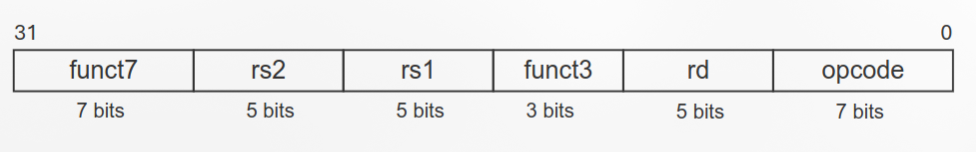
\includegraphics{images/rtype.png}
    \caption{R-type Instructions}
    \label{fig:rtype}
\end{figure}
\begin{itemize}
    \item \texttt{opcode}: partially specifies instruction
    \item \texttt{funct7 + funct3}: combined with opcode, specifies what operation
    \item \texttt{rs1}: first operand (source register 1)
    \item \texttt{rs2}: second operand (source register 2)
    \item \texttt{rd}: destination register (receives the result of the computation)
\end{itemize}
For example, the operation \texttt{x9, x20, x21}
is \texttt{0x015A04B3}.

I-type instructions are immediate arithmetic
and load instructions, and have the form given
in Figure \ref{fig:itype}.
\begin{figure}
    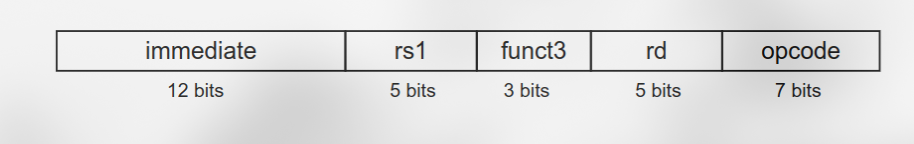
\includegraphics{images/itype.png}
    \caption{I-type Instructions}
    \label{fig:itype}
\end{figure}
\begin{itemize}
    \item \texttt{rs1}: source or base address register number.
    \item \texttt{immediate}: constant operand, or offset added to base address.
\end{itemize}

S-type instructions have the form in
Figure \ref{fig:stype}
\begin{figure}
    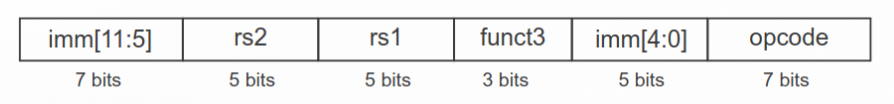
\includegraphics{images/stype.png}
    \caption{S-type Instructions}
    \label{fig:stype}
\end{figure}
\begin{itemize}
    \item \texttt{rs1}: base address register number
    \item \texttt{rs2}: source operand register number
    \item \texttt{immediate}: offset added to base address
\end{itemize}

